%
%===============>>  Кузнецов Модуль 8 <<=============
%=
\setmodule{8}

%BEGIN_FOLD % ====>>_____ Занятие 1 _____<<====
\begin{class}[number=1]
	\begin{listofex}
		\item 
		\begin{tasks}(1)
			\task Решите уравнение \( \cos2x+sin^2x=0,75 \)
			\task Найдите все корни этого уравнения, принадлежащие отрезку \( \left[ -3\pi; -\dfrac{3\pi}{2}\right] \) 
		\end{tasks}
		\item 
		\begin{tasks}(1)
			\task Решите уравнение: \( 6\sin^2x+15\sin\left( \dfrac{3\pi}{2}+x \right)-12=0 \)
			\task Найдите все корни этого уравнения, принадлежащие отрезку \( \left[ -5\pi; -\dfrac{7\pi}{2}\right] \) 
		\end{tasks}
		\item 
		\begin{tasks}(1)
			\task Решите уравнение \( \sin2x+\sqrt{3}\sin x=0 \)
			\task Найдите все корни этого уравнения, принадлежащие отрезку \( \left[ \dfrac{5\pi}{2}; \dfrac{7\pi}{2}\right] \) 
		\end{tasks}
		\item 
		\begin{tasks}(1)
			\task Решите уравнение \( 4\sin^3x=3\cos\left( x-\dfrac{\pi}{2} \right) \)
			\task Найдите все корни этого уравнения, принадлежащие отрезку \( \left[ \dfrac{7\pi}{2}; \dfrac{9\pi}{2}\right] \) 
		\end{tasks}
		\item 
		\begin{tasks}(1)
			\task Решите уравнение \( \cos2x=1-\cos\left( \dfrac{\pi}{2}-x \right) \)
			\task Найдите все корни этого уравнения, принадлежащие отрезку \( \left[ -\dfrac{5\pi}{2}; -\pi\right] \) 
		\end{tasks}
		\item 
		\begin{tasks}(1)
			\task Решите уравнение \( 4\sin^3x=3\cos\left( x-\dfrac{\pi}{2} \right) \)
			\task Найдите все корни этого уравнения, принадлежащие отрезку \( \left[ \dfrac{7\pi}{2}; \dfrac{9\pi}{2}\right] \) 
		\end{tasks}
		\item 
		\begin{tasks}(1)
			\task Решите уравнение \( \dfrac{1}{\sin^2x}-\dfrac{3}{\sin x}+2=0 \)
			\task Найдите все корни этого уравнения, принадлежащие отрезку \( \left[ -\dfrac{5\pi}{2}; -\pi\right] \) 
		\end{tasks}
		\item 
		\begin{tasks}(1)
			\task Решите уравнение \( \sin(\pi-x)-\cos\left( \dfrac{\pi}{2}+x \right)=-1 \)
			\task Найдите все корни этого уравнения, принадлежащие отрезку \( \left[ -\pi; \dfrac{3\pi}{2}\right] \) 
		\end{tasks}
	\end{listofex}
\end{class}
%END_FOLD

%BEGIN_FOLD % ====>>_____ Занятие 2 _____<<====
\begin{class}[number=2]
	\begin{listofex}
		\item Площадь параллелограмма равна \( 54 \), две его стороны равны \( 18 \) и \( 36 \). Найдите большую высоту этого параллелограмма.
		\item В правильной треугольной пирамиде \( SABC \) медианы основания \( ABC \) пересекаются в точке \( O \). Площадь треугольника \( ABC \) равна \( 9 \); объем пирамиды равен \( 6 \). Найдите длину отрезка \( OS \).
		\item При производстве в среднем из \( 2000 \) насосов \( 4 \) неисправных. Найдите вероятность того, что случайно выбранный насос окажется неисправным.
		\item Симметричную монету бросают \( 10 \) раз. Во сколько раз вероятность события «выпадет ровно \( 5 \) орлов» больше вероятности события «выпадет ровно \( 4 \) орла»?
		\item Найдите корень уравнения: \( \left( \dfrac{1}{5} \right)^{x-6}=125 \)
		\item Найдите значение выражения: \( \dfrac{\log_318}{2+\log_32} \)
		\item На рисунке изображен график производной функции \( f(x) \), определенной на интервале \( (-13; 10) \). Найдите количество точек минимума функции \( f(x) \) на отрезке \( [-9;9] \).
		\begin{center}
			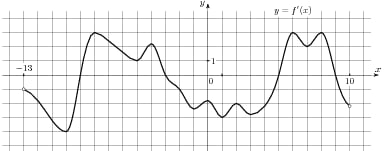
\includegraphics[align=t, width=0.8\linewidth]{../\picpath/KuznetsovM8L2}
		\end{center}
		\item При адиабатическом процессе для идеального газа выполняется закон \(pV^k=10^5\)Па\(\cdot\)м\(^5\), где \(p\) --- давление газа в паскалях, \(V\) --- объeм газа в кубических метрах, \(k=\dfrac{  5}{ 3 }\).  Найдите, какой объём \(V\) (в куб. м) будет занимать газ при давлении \(p\), равном \(3,2\cdot10^6\) Па.
		\item Имеется два сплава. Первый сплав содержит \( 5\% \) меди, второй --- \( 12\% \) меди. Масса второго сплава больше массы первого на \( 9 \) кг. Из этих двух сплавов получили третий сплав, содержащий \( 10\% \) меди. Найдите массу третьего сплава. Ответ дайте в килограммах.
		\item
		\begin{minipage}[t]{\bodywidth}
			На рисунке изображён график функции вида \(f(x)= a^x\). Найдите значение \(f(3)\).
		\end{minipage}
		\begin{minipage}[t]{\picwidth}
			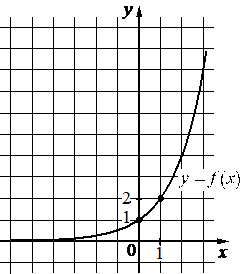
\includegraphics[align=t, width=\textwidth]{../\picpath/G111M8L6-2}
		\end{minipage}
		\item Найдите точку минимума функции \( y=(x+16)e^{x-16} \).
	\end{listofex}
	\begin{listofex}
		\item Острый угол ромба равен \( 30\degree \). Радиус вписанной в этот ромб окружности равен \( 2 \). Найдите сторону ромба.
		\item
		\begin{minipage}[t]{\bodywidth}
			Найдите объем пространственного креста, изображенного на рисунке и составленного из единичных кубов.
		\end{minipage}
		\begin{minipage}[t]{\picwidth}
			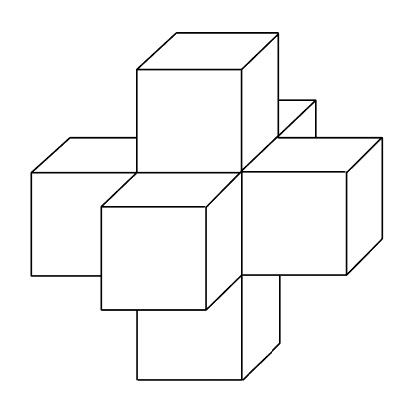
\includegraphics[align=t, width=\textwidth]{../\picpath/G101M5L7-4}
		\end{minipage}
		\item В группе туристов \( 32 \) человека. Их вертолётом в несколько приёмов забрасывают в труднодоступный район по \( 4 \) человека за рейс. Порядок, в котором вертолёт перевозит туристов, случаен. Найдите вероятность того, что турист К. полетит пятым рейсом вертолёта.
		\item Вероятность того, что новый тостер прослужит больше года, равна \( 0,94 \). Вероятность того, что он прослужит больше двух лет, равна \( 0,8 \). Найдите вероятность того, что он прослужит меньше двух лет, но больше года.
		\item Решите уравнение: \( \sqrt{\dfrac{1}{15-4x}}=0,2 \)
		\item Найдите значение выражения: \( ((2x^3)^4-(x^2)^6):(3x^{12}) \)
		\item 
		\begin{minipage}[t]{\bodywidth}
			На рисунке изображены график функции \( y=f(x) \) и касательная к этому графику, проведённая в точке \( x_0=2 \). Найдите значение производной функции \( g(x)=x^2-f(x)+1 \) в точке \( x_0 \).
		\end{minipage}
		\begin{minipage}[t]{\picwidth}
			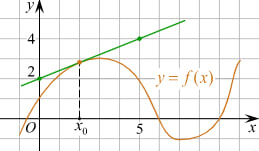
\includegraphics[align=t, width=\textwidth]{../\picpath/KuznetsovM8L2_1}
		\end{minipage}
		\item Два тела массой \(m=2\) кг каждое, движутся с одинаковой скоростью  \(v =10\) м/с под углом \(2\alpha\) друг к другу. Энергия (в джоулях), выделяющаяся при их абсолютно неупругом соударении определяется выражением \(Q= m v^2 \sin^2 \alpha \). Под каким наименьшим углом \(2\alpha\) (в градусах) должны двигаться тела, чтобы в результате соударения выделилось не менее \(50\) джоулей?
		\item На изготовление \( 588 \) деталей первый рабочий затрачивает на \( 7 \) часов меньше, чем второй рабочий на изготовление \( 672 \) деталей. Известно, что первый рабочий за час делает на \( 4 \) детали больше, чем второй. Сколько деталей в час делает первый рабочий?
		\item
		\begin{minipage}[t]{\bodywidth}
			На рисунке изображен график функции \( f(x)=\dfrac{x^2}{a}+bx+c \). Найдите \( f(4) \).
		\end{minipage}
		\begin{minipage}[t]{\picwidth}
			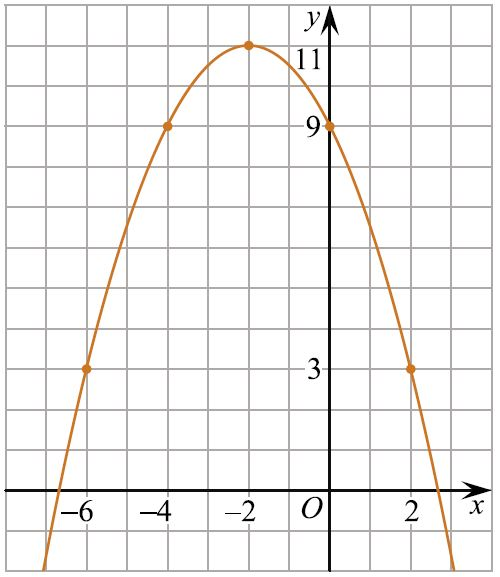
\includegraphics[align=t, width=\textwidth]{../\picpath/G112M3C2-4}
		\end{minipage}
		\item Найдите наименьшее значение функции \( y=(x-7)^2(x-6)+6 \) на отрезке \( [6,5;19] \).
	\end{listofex}
\end{class}
%END_FOLD

%BEGIN_FOLD % ====>>_ Домашняя работа 1 _<<====
\begin{homework}[number=1]
	\begin{listofex}
		\item Домашняя работа 1
	\end{listofex}
\end{homework}
%END_FOLD

%BEGIN_FOLD % ====>>_____ Занятие 3 _____<<====
\begin{class}[number=3]
	\begin{listofex}
		\item Занятие 3 
	\end{listofex}
\end{class}
%END_FOLD

%BEGIN_FOLD % ====>>_____ Занятие 4 _____<<====
\begin{class}[number=4]
	\begin{listofex}
		\item Занятие 4
	\end{listofex}
\end{class}
%END_FOLD

%BEGIN_FOLD % ====>>_ Домашняя работа 2 _<<====
\begin{homework}[number=2]
	\begin{listofex}
		\item Домашняя работа 2
	\end{listofex}
\end{homework}
%END_FOLD

%BEGIN_FOLD % ====>>_____ Занятие 5 _____<<====
\begin{class}[number=5]
	\begin{listofex}
		\item Занятие 5
	\end{listofex}
\end{class}
%END_FOLD

%BEGIN_FOLD % ====>>_____ Занятие 6 _____<<====
\begin{class}[number=6]
	\begin{listofex}
		\item Занятие 6
	\end{listofex}
\end{class}
%END_FOLD

%BEGIN_FOLD % ====>>_ Домашняя работа 3 _<<====
\begin{homework}[number=3]
	\begin{listofex}
		\item Домашняя работа 3
	\end{listofex}
\end{homework}
%END_FOLD

%BEGIN_FOLD % ====>>_____ Занятие 7 _____<<====
\begin{class}[number=7]
	\title{Подготовка к проверочной}
	\begin{listofex}
		\item Занятие 7
	\end{listofex}
\end{class}
%END_FOLD

=%BEGIN_FOLD % ====>>_ Проверочная работа _<<====
\begin{exam}
	\begin{listofex}
		\item Проверочная
	\end{listofex}
\end{exam}
%END_FOLD